%!TEX root = ../../dissertation.tex
%%%%%%%%%%%%%%%%%%%%%%%%%%%%%%%%%%%%%%%%%%%%%%%%%%%%%%%%%%%%%%%%%%%%%%%%%%%%%%%
\section{Modeling Mobile Network Load}
\label{c4:modeling}

Drawing conclusions from statistical analysis alone is a difficult task. The next logical step lies therefore in the creation of models abstracting this real system, making them easier to calculate with the loss of some precision. This and future improved models should support network operators in predicting the signaling load in their core network with the benefit of improved network engineering and correctly scaling core components.


%%%%%%%%%%%%%%%%%%%%%%%%%%%%
% intro part from MMB 2014
%\section{Introduction}

With the increased importance of smart phones, mobile networks are currently experiencing rapid growth.
Compared to a fixed access provider additional aspects have to be taken into account when dimensioning a mobile network. 
First and most prominent is the planning of radio access cells --- their coverage, frequency selection,  and backhaul, i.e. connection to the operator's network. Aside from substantial administrative and financial efforts this problem has been largely solved, radio network planning tools and research readily exists \cite{tutschku1998demand}.
Albeit of equal importance, there is much less public knowledge and research on the second aspect in setting up the mobile network: dimensioning the core network. Consisting of a large number of specialized network nodes not available as of-the-shelf commodity hardware and in need of careful tuning to each other, correctly putting together the core is no small feat. Unlike fixed access, mobile access networks require much more state to be held, with the nodes having to signal any state-change throughout the network.

One major metric to consider in the dimensioning is the number of supported tunnels, i.e. connections to the Internet, of the \gls{GGSN}.
The performance requirements of the \gls{GGSN} depend on factors like customers to serve, applications in the network, user behavior and devices used. These factors are, during dimensioning, either unknown or subject to change as user behavior evolves.
But these network components are sold as static middleboxes and cannot not be easily extended with of-the-shelf hardware in order to account for new requirements.
The newly introduced concept of \gls{NFV} \cite{nfv_whitepaper} suggests to harness technologies from cloud computing in the network. This would allow network operators to scale out, i.e. using additional low performance machines, instead of scaling up, which requires them to replace existing hardware with more powerful components.

The contribution of this work is threefold. First, we introduce models for both a traditional \gls{GGSN} as well as a virtual \gls{GGSN} using \gls{NFV}. Secondly, we provide distributions for \gls{gtp} tunnel interarrival times and durations, readily to be used in other studies. Finally, we study performance trade-offs when using a virtual \gls{GGSN}, discussing different options to consider when using a virtual \gls{GGSN}.


%%%%%%%%%%%%%%%%%%%%%%%%%%%%%%%%%%%%%%%%%%%%%%%%%%%%%%%%%%%%%%%%%%%%%%%%%%%%%%%
\subsection{Creating a Simple Toy Queuing Model}

\begin{figure}[htb]
	\centering
	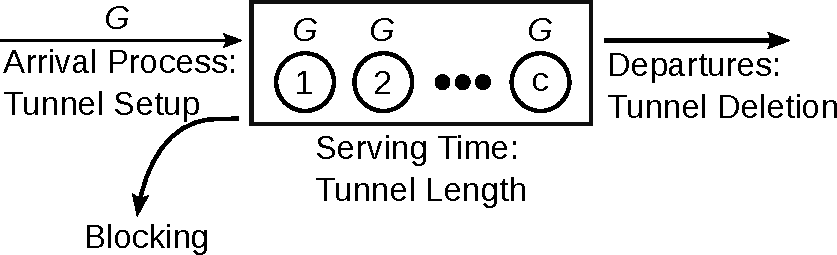
\includegraphics[width=\columnwidth]{images/GGn-model.pdf}
	\caption{Simple toy-model for tunnel-induced load on the core network.}
	\label{c4:fig:ggn-model}
\end{figure}

To begin the modeling process we attempt to represent the tunnel management as a queuing system, specifically as a G/G/n-0 system in Kendall's notation. Figure~\ref{c4:fig:ggn-model} shows this model for the case of our proposed tunnel load metric. Here, tunnels enter the system by a general random distribution, are then ``served'' at the \gls{GGSN} for the duration of their existence, which also follows a general distribution, and leave the system, i.e. are torn down, afterwards. If the serving units are filled, blocking occurs and arriving tunnel requests are rejected.

In this case ``servers'' correspond to available resources at one or more \gls{GGSN}, making the maximum number of tunnels hard to guess and depend on a number of factors. This could include soft-limits like the specific configuration, and hard-limits, e.g. the \gls{GGSN}'s processing and memory constraints. Unfortunately, all of these are unknown to us. Moreover, as the tunnels are all served on a relatively small number of hardware entities they are not independent of each other. Increasing load could very well influence both the arrival as well as the serving process.

For the purpose of creating a toy model we are further simplifying the $G/G/n-0$ to a $M/M/\infty$ queue. As stated, no actual limit to the number of virtual servers is known and the data also does not show any obvious limits. So we can safely assume an unlimited system and do not have to treat blocking or queuing explicitly.

\begin{figure}[htb]
	\centering
	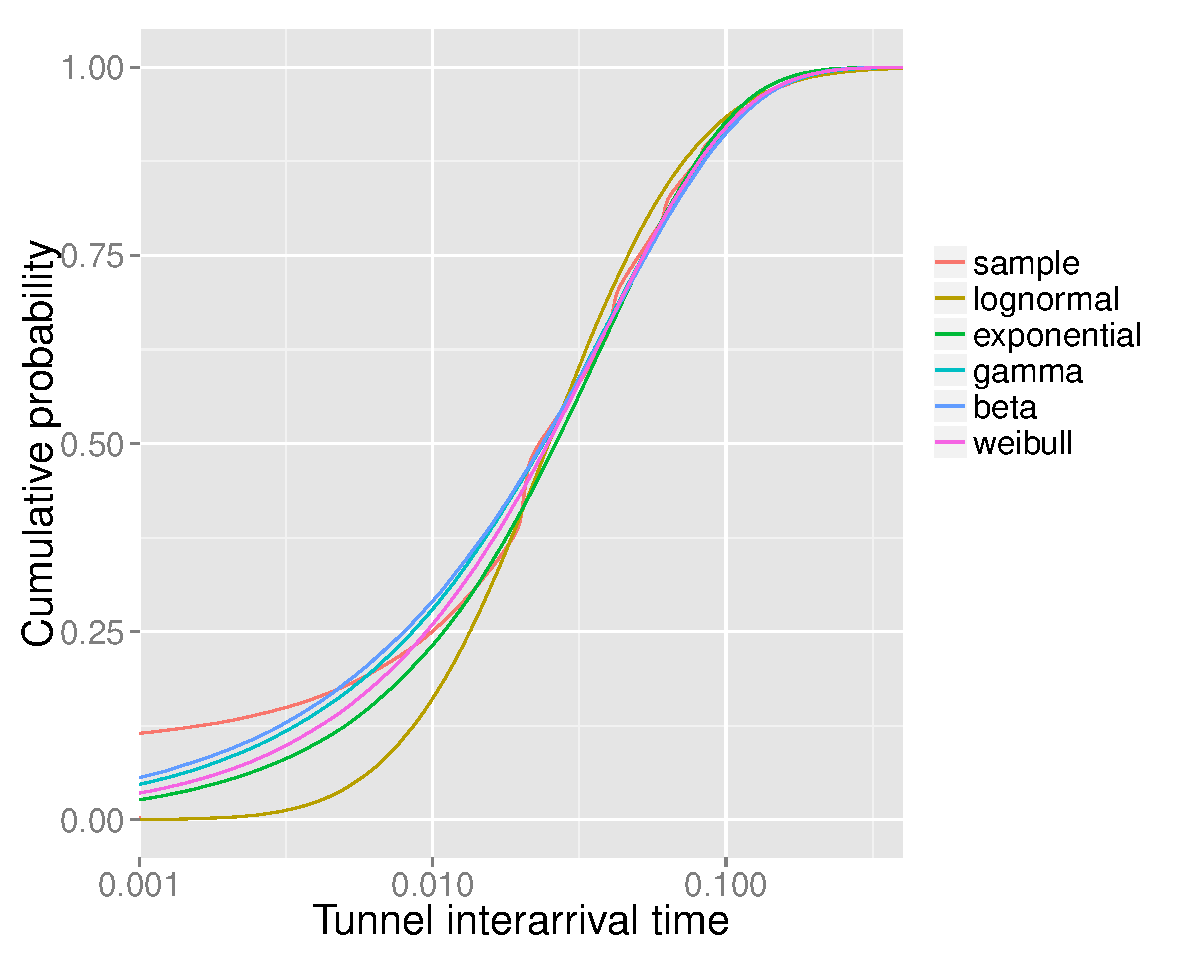
\includegraphics[width=\columnwidth]{images/R-IAT-ecdfs.pdf}
	\caption{Sampled inter-arrival time CDF and fitted theoretical distributions.}
	\label{c4:fig:IAT-cdfs}
\end{figure}

Furthermore, we fitted univariate distributions to the experimental data for the tunnel inter-arrivals and durations and tested the goodness of the fit both numerically, using Pearson's $\chi^2$ test, and visually for the density and CDF plots. No standard random distribution reaches the significance level for either process. We attribute this fact largely to the various artifacts in the data, e.g. the described wave effect every \SI{20}{\milli\second} in the inter-arrival time. Matching them visually (confer also the cumulative distribution function plot in Figure~\ref{c4:fig:IAT-cdfs}) we find that the exponential fit is reasonably close to the experimental data in both the arrival and duration cases. Again, these distribution fits are just for a toy model to lay the groundwork for future and improved modeling.


\begin{figure}[htb]
	\centering
	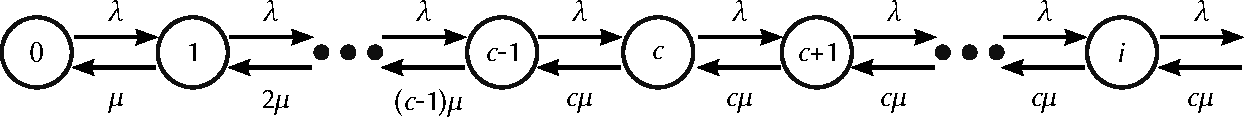
\includegraphics[width=\columnwidth]{images/markovchain.pdf}
	\caption{Markov chain model for the tunnel serving process.}
	\label{c4:fig:markovchain}
\end{figure}

Now, assuming both a Poisson arrival and an exponential serving process, a Markov chain representing the queue can be set up (cf. Fig.~\ref{c4:fig:markovchain}) and stationary analysis can be conducted. From the measured data an arrival rate of $\lambda=25.64123$ and the parameter $\mu=0.0001586728$ for the exponential service time distribution are calculated. Using Little's Law this gives an estimate for the mean number of concurrent tunnels at the \gls{GGSN} of 

$$
L=\frac{\lambda}{\mu}\approx 161\,599. %=161598.14.
$$

As stated, the amount of state held at the node and propagated through the network is directly related to the number of tunnels. Therefore, we propose this metric as an initial estimate of the load at the \gls{GGSN}.


%%%%%%%%%%%%%%%%%%%%%%%%%%%%%%%%%%%%%%%%%%%%%%%%%%%%%%%%%%%%%%%%%%%%%%%%%%%%%%%
\subsection{Advanced Models} 


On the basis of this toy model better fitting models can now be constructed. Those should also factor in more of the core network's properties and specified parameters omitted in this model. Specifically, this means shifting from $M/M/\infty$ to the more generalized $G/G/n$ and therefore finding better distribution fits for the involved processes.

It is also entirely possible that the single queue approach is not the best way to describe control plane load. Several load influencing factors discussed earlier have direct influence on the tunnel arrivals and duration, e.g. the device type or the radio access technology. Therefore, amongst others multidimensional queuing networks or fluid flow could be a better fit. Our plan is to conduct further investigations into the modeling of mobile core network signaling. This also includes a rough simulative approach, which could also be used to validate our models against experimental data.


%%
\subsubsection{Monolithic \texorpdfstring{\acrshort{GGSN}}{GGSN}}

In this section we provide a model for a traditional \gls{GGSN} and discuss a model for a virtual \gls{GGSN} using \gls{NFV}. In \gls{NFV} \cite{nfv_whitepaper} static network middleboxes are replaced by commodity hardware. The tasks solved by the original middleboxes are then solved by dediciated software.

\begin{figure}[htb]
  \centering
  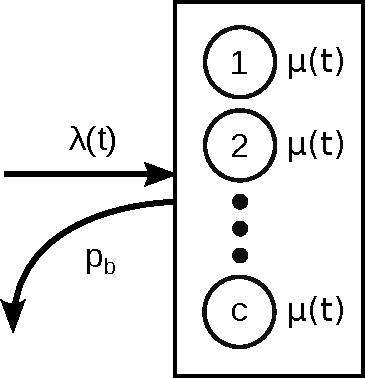
\includegraphics[width=0.6\textwidth]{images/ggsn-monolithic.pdf}
  \caption{Model of a Traditional GGSN}
  \label{fig:model_traditional_ggsn}
\end{figure}

First, we give a model for a \emph{traditional} \gls{GGSN}, i.e. a network static network component.
While we consider the \gls{GGSN} to be one fixed entity, it can in reality consist of multiple servers. However, due to the fact that the \gls{GGSN} is purchased from a vendor as a middlebox, idle servers can be neither deactivated nor reused for other purposes.

The queuing theory equivalent is displayed in Figure~\ref{fig:model_traditional_ggsn}. New tunnels requests arrive according to a Poisson distribution with a rate of $\lambda(t)$ at the \gls{GGSN}. This server will have a maximum tunnel capacity of $c_c$. When it is reached, blocking will occur and newly incoming tunnels are rejected. Traditionally, \glspl{GGSN} can be expected to be overdimensioned in such a way, that this rarely happens. If the new tunnel is accepted, it will occupy one of the serving units of the unit for the duration $\mu(t)$ of the tunnel. As stated earlier, we can not model the tunnel duration to be markovian, resulting in a  $M/G/c_c$ loss system. In order to give quality of service guarantees the network operator is interested in the system's blocking probability $p_B$, which we consider to be a key metric of our model. Additionally, the previously described diurnal patterns can are also be modeled by adjusting the arrival and serving process distributions for each time of day. This alternatively also allows just to investigate the busy hour and thus the system's peak load.


%%
\subsubsection{\texorpdfstring{\acrshort{GGSN}}{GGSN} using Network Function Virtualization}
\label{c4:sec:virtual_ggsn}

\begin{figure}[htb]
  \centering
  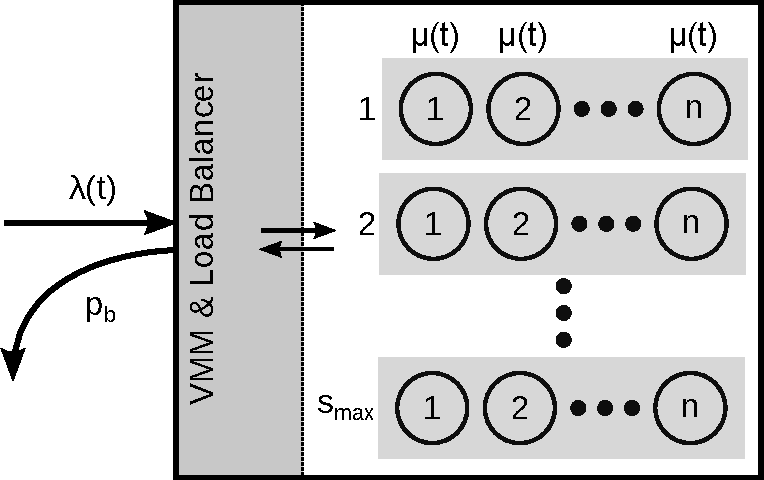
\includegraphics[width=0.7\textwidth]{images/ggsn-virtualized.pdf}
  \caption{Model of a GGSN using Network Function Virtualization}
  \label{c4:fig:model_nfv_ggsn}
\end{figure}

In the second model, we introduce concepts from \gls{NFV}, i.e. the idea to replace middleboxes with commodity hardware. This allows us to realize benefits from cloud computing, as we are now able to scale out, instead of up. The assumptions of the Markov arrival process $\lambda(t)$ and the serving time distributions $\mu(t)$ are carried over. However, instead of one server processing every tunnel, this model assumes that there are up to $s_{max}$ virtualized servers $s_i$. Each of these is much smaller than the traditional \gls{GGSN}, having a tunnel serving capacity of $c_i \ll c_c$ and a total system capacity of $c_{max} = s_{max} \times i$.

In its initial state, for efficiency, all but a small portion of the server instances should be shut of. Only, when a certain condition is reached, a new one is provisioned. As a simple example, one could always hold one instance in reserve for upcoming requests and provision as soon as the reserver gets used. Similar rules should apply in the shutdown of servers and should form a hysteresis together with the boot condition. For example it would be possible to keep at least one server in reserve but never more than two.

If these conditions are not carefully selected and are in tune with the expected boot time of an instance, additional blocking can occur. Despite not having reached its maximum capacity, this system will still reject tunnel requests during the provisioning phase when no tunnel slots are free. This could be remedied by a request queue. However, this might just make the system more complex without providing real benefit, as mobile devices usually will repeat their attempts and would time out anyway when the request is taking too long. 

To place incoming tunnel state on one of the available servers a load balancer is required. To ensure, that the system in run time can scale down to its actual needs, the balancer should place tunnels on servers, that are the fullest, keeping the reserve free. It may even migrate tunnel state from almost empty servers away so that these can be shut down, when the condition is fulfilled. Keeping instance close to their capacity should also have no impact on the performance a mobile device associated to a specific tunnel experiences. Adequate strategies for both load balancing and migration will be considered in future work.




%%%%%%%%%%%%%%%%%%%%%%%%%%%%%%%%%%%%%%%%%%%%%%%%%%%%%%%%%%%%%%%%%%%%%%%%%%%%%%%
\subsection{Simulative Validation} 


%%
\subsubsection{Testing the Model Numerically}
\label{c4:sec:model-numerical}

We implement the models using a \gls{DES} with the SimPy \cite{simpy} package as foundation. Our implementation is also publicly available\footnote{\url{https://github.com/fmetzger/ggsn-simulation/}} as a reference for future publications. To be in line with the measurement data we consider a simulation time of 7 days for all simulation scenarios, with a transient phase of \SI{60}{\minute} accounted for. Ten replications of each scenario were performed. All error bars given in this section show the \SI{5}{\percent} and \SI{95}{\percent} quantiles of all replications.


We use the measurements in order to dimension a traditional \gls{GGSN} as a baseline for all further studies. Based on these results, we examine the effects of network function virtualization by scaling \emph{out} instead of up through a virtual \gls{GGSN} model. Finally, we arrive at a more realistic version of the virtual \gls{GGSN} by taking the start up and shut down times into account.


%%
\subsubsection{Queuing Simulation Implementation}


%%
\subsubsection{Traditional GGSN}
\label{c4:sec:eval_traditional_ggsn}

With the help of the interarrival times and duration of tunnels we study the traditional \gls{GGSN} model previously introduced. Whilst our measurements provided us with information on the frequency of new tunnels and the duration they remain active, we have no reliable information on the number of active tunnels the \gls{GGSN} can support. Thus, in a first step, we dimension the \gls{GGSN} in such a way that a suitable blocking probability $p_B$ can be achieved.

\begin{figure}[htp]
  \centering
    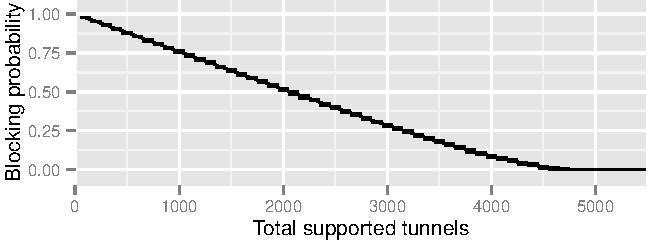
\includegraphics[width=1.0\textwidth]{images/traditional-blocking.pdf}
  \caption{Impact of the number of supported parallel tunnels on the blocking probability for the traditional \gls{GGSN} model. For each scenario the mean of all simulated replications as well as \SI{5}{\percent} and \SI{95}{\percent} quantiles as error bars are shown.}
  \label{c4:fig:traditional_blocking}
\end{figure}

In Figure~\ref{c4:fig:traditional_blocking} the maximum number of tunnels $n$, that can be active simultaneously, is gradually increased to study the impact on the blocking probability $p_B$. We observe, that as the number of supported parallel tunnels increases, the blocking probability decreases. For the normalized interarrival no blocking is occurring if we allow for more than $5000$ parallel tunnels. Thus, we consider the range of $4000$ to $5000$ parallel tunnels to be of special interest for the remainder of the study.


%%
\subsubsection{Virtual \texorpdfstring{\acrshort{GGSN}}{GGSN}}
\label{c4:sec:eval_ideal_virtual_ggsn}

In order to study the feasibility of the virtual \gls{GGSN} approach discussed in Sec.~\ref{c4:sec:virtual_ggsn}, we compare the performance indicators of the virtual \gls{GGSN} with that of a traditional \gls{GGSN}. To this end, the virtual \gls{GGSN} is simulated in varying configurations.
The number of servers and supported tunnels per server is chosen in such a way that the results can be compared with those obtained from our study of the traditional \gls{GGSN}. Due to simulation time constraints, only a representative subset of scenarios is simulated.

In the virtual \gls{GGSN} model, servers are activated and deactivated on demand, while in the traditional \gls{GGSN} model, the single server is always on. For this investigation a conservative start up and shut down time of \SI{300}{\second} is chosen. Generally, deactivating server instances reduces energy consumption and frees up inactive servers for other use. For this reason, the number of active servers is a relevant performance metric in the virtual \gls{GGSN} model.


\begin{table}[htp]
	\caption{Manipulation check for the experimental factors based on one-way ANOVA.}
	\centering
	\label{c4:tab:manipulation2color}
	\begin{tabu}{X[l]X[r]X[r]X[r]XX}%{lrrrcc}
	\toprule
	& \multicolumn{1}{c}{$\mathbf{F(2,1275)}$} & \multicolumn{1}{c}{$\mathbf{\eta^2_p}$} & \multicolumn{1}{c}{$\mathbf{p}$} & \textbf{Cohen's} & \textbf{Cohen's}\\ 
	&  & & & $\mathbf{f^2}$ & $\mathbf{\hat{\omega}^2}$ \\ 
	\midrule
	\emph{blocking probability}  & & & & &\\ 
	maxTunnels &  $15601.534$ & $\color{red} 0.99$ & $<0.001$ & $\color{red} 26.739$ & $0.964$\\ 
	maxInstances &  $10218.173$ & $\color{red} 0.986$ & $<0.001$ & $\color{red} 1.068$ & $0.516$\\ 
	startstopDuration &  $0.868$ & $\color{black} 0.003$ & $0.482$ & $\color{black} 0.000$ & $0.000$\\ 
	\midrule
	\emph{mean number of tunnels}  & & & & &\\ 
	maxTunnels &  $20448.347$ & $\color{red} 0.994$ & $<0.001$ & $\color{red} 27.712$ & $0.965$\\ 
	maxInstances &  $13348.251$ & $\color{red} 0.989$ & $<0.001$ & $\color{red} 1.064$ & $0.515$\\ 
	startstopDuration &  $2.872$ & $\color{black} 0.009$ & $0.022$ & $\color{black} 0.000$ & $0.000$\\ 
	\bottomrule
	\end{tabu}
\end{table}

In order to analyze the influence of the different model parameters on the performance metrics, we perform a one-way ANOVA analysis with the results in Table~\ref{c4:tab:manipulation2color}. High values for $\eta_p^2$ and Cohen's $f^2$ \cite{stats} indicate that the main influence for both blocking probability and mean number of tunnels is the maximum number of tunnels $n$ and servers $S_{\max}$, i.e. the total number of possible concurrent tunnels in the system.
Therefore, we study these parameters first.

\begin{figure}[htb]
  \centering
  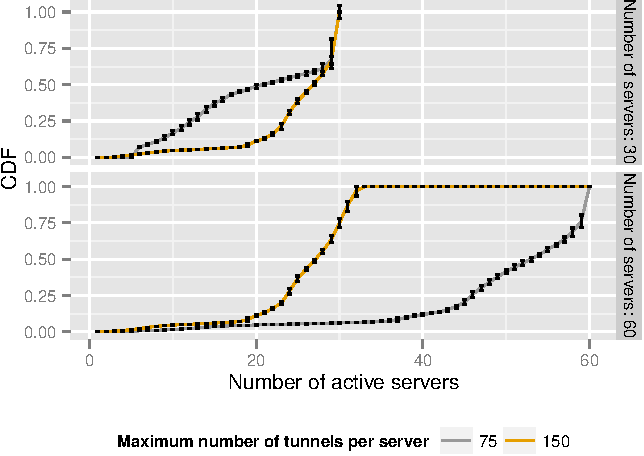
\includegraphics{images/instanceuse-multiserver-real.pdf}
  \caption{Impact of the maximum number of tunnels and number of servers on number of active servers in the virtual \gls{GGSN} model.}
 \label{c4:fig:instance_use_virtual}
\end{figure}

In Figure~\ref{c4:fig:instance_use_virtual} the \gls{CDF} of the number of active servers for four different virtual \gls{GGSN} configurations is displayed. We observe, that increasing the number of supported tunnels per server allows a larger percentage of servers to be shutdown or used for other tasks. This demonstrates the scaling capability of the virtualized model quite well. Note, that both the scenario with $30$ servers and $150$ maximum tunnels per server as well as the scenario with $60$ servers and $75$ maximum tunnels per server share the same maximum amount of tunnels, $4500$, being right at the center of the interesting range of candidates.


\begin{figure}[htb]
  \centering
  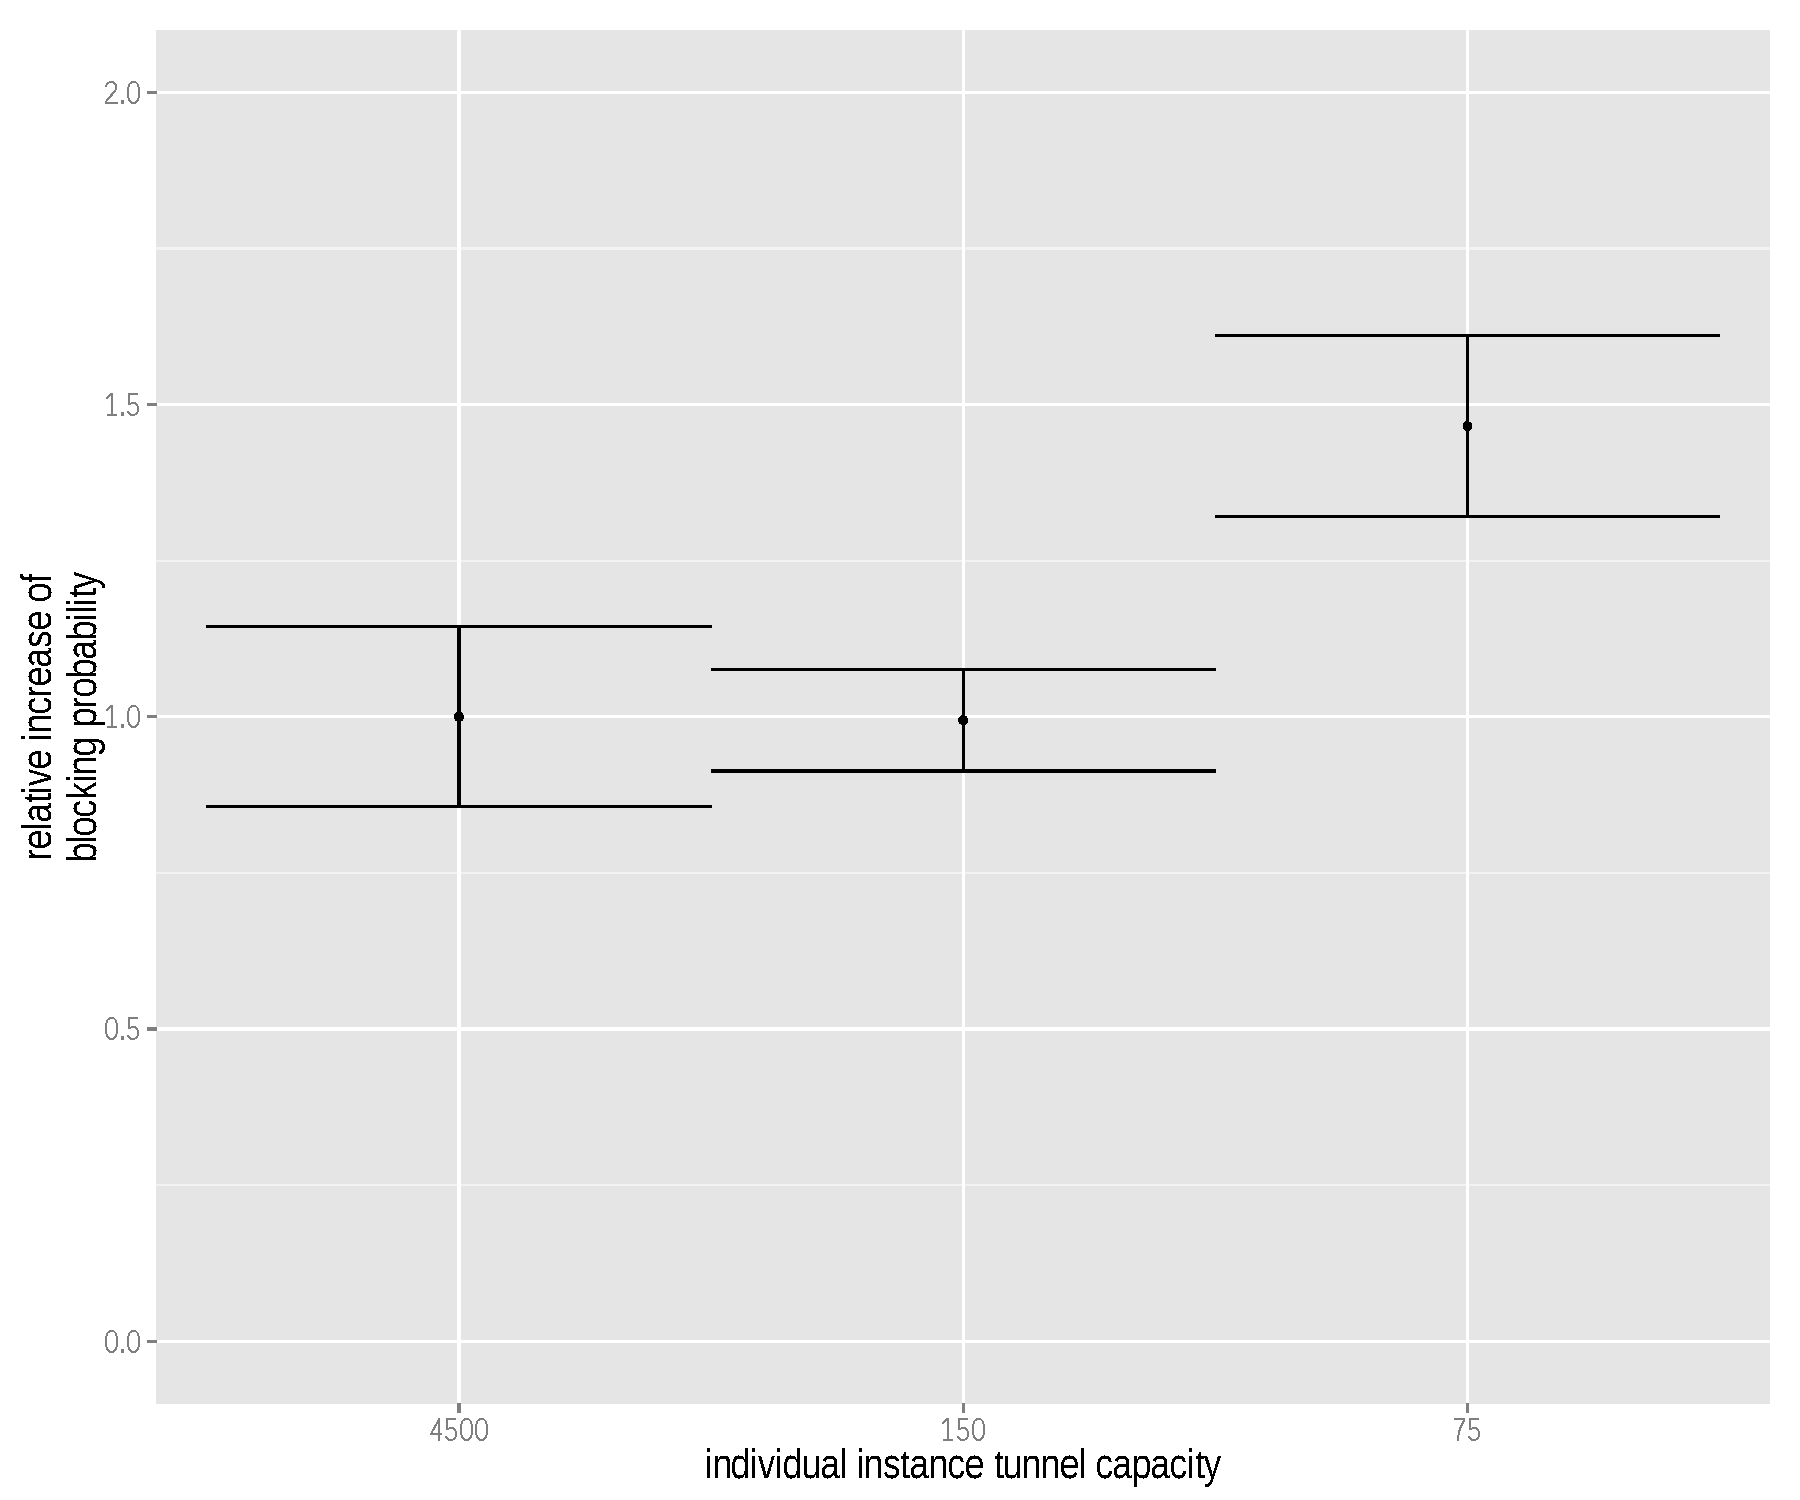
\includegraphics{images/blocking-comparison.pdf}
  \caption{Relative increase of blocking probability on the number of servers compared to the traditional \gls{GGSN}; with the $4500$ maximum tunnels per server being on a single server, $150$ on $30$, and $75$ on $60$ servers.}
 \label{c4:fig:blocking-comparison}
\end{figure}

Next, we take a look at the blocking probability of the virtual \gls{GGSN} system in Figure~\ref{c4:fig:blocking-comparison} and compare it to the results from the traditional \gls{GGSN} model. In Figure~\ref{c4:fig:blocking-comparison} we compare the blocking probability of the traditional \gls{GGSN} system dimensioned for $4500$ concurrent tunnels with the virtual \gls{GGSN}.

We observe that, with the start up and shut down time of $5$ minutes in mind, the blocking probability increases by a factor of $1.48$ if the capacity of each server is set to $75$, i.e. $\frac{1}{60}$ of the original server capacity, while $27$ of all $60$ servers can be turned of or used for other purposes at \SI{50}{\percent} of the time. We conclude, that choosing more powerful servers decreases the blocking probability but reduces the potential to disable servers.

So far we have considered a conservative start up and shut down time of servers of \SI{5}{\minute}, which can potentially occur if current generation physical servers are used.
In the next section we study the impact of reduced start up and shut down times with modern servers with fast storage (e.g. \glspl{SSD}) or virtual servers provisioned in the cloud.


%%
\subsubsection{Impact of startup and shutdown times}
\label{c4:sec:real_virtual_ggsn}

In this section, we first consider the impact of different boot and shut down times on resource utilization and blocking probabilities. We observe the impact of different start up and shut down times on both resource utilization and blocking probability. Afterwards, the influence of varying server start and stop times on a fixed combination of maximum tunnels and servers in the system is examined.

\begin{figure}[htb]
  \centering
  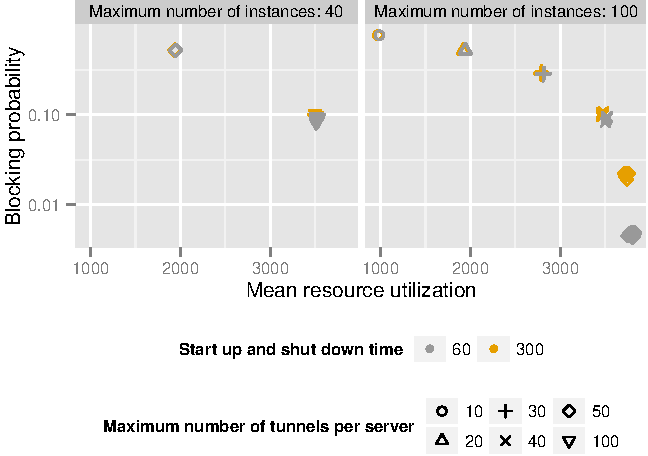
\includegraphics{images/compare-util-block.pdf}
  \caption{Trade-off between blocking probability and mean resource utilization with regard to maximum number of servers, maximum number of tunnels per server, and start up and shut down time.}
 \label{c4:fig:compare_util_block}
\end{figure}

Figure~\ref{c4:fig:compare_util_block} shows scenarios with $40$ and $100$ number of virtual \gls{GGSN} instances and  $1000$ to $5000$ total concurrent tunnels. For each scenario, we study the impact of selecting different maximum numbers of tunnel per server as well as start up and shut down times on blocking probability and mean resource utilization. The first observation is that by increasing the number of servers, i.e. scaling out, the blocking probability can be decreased, while maintaining a relatively low mean resource utilization. In addition to the previous effects, we notice that a higher start up and shut down time causes a slight increase in blocking probability for servers with low tunnel capacity.

\begin{figure}[htb]
  \centering
  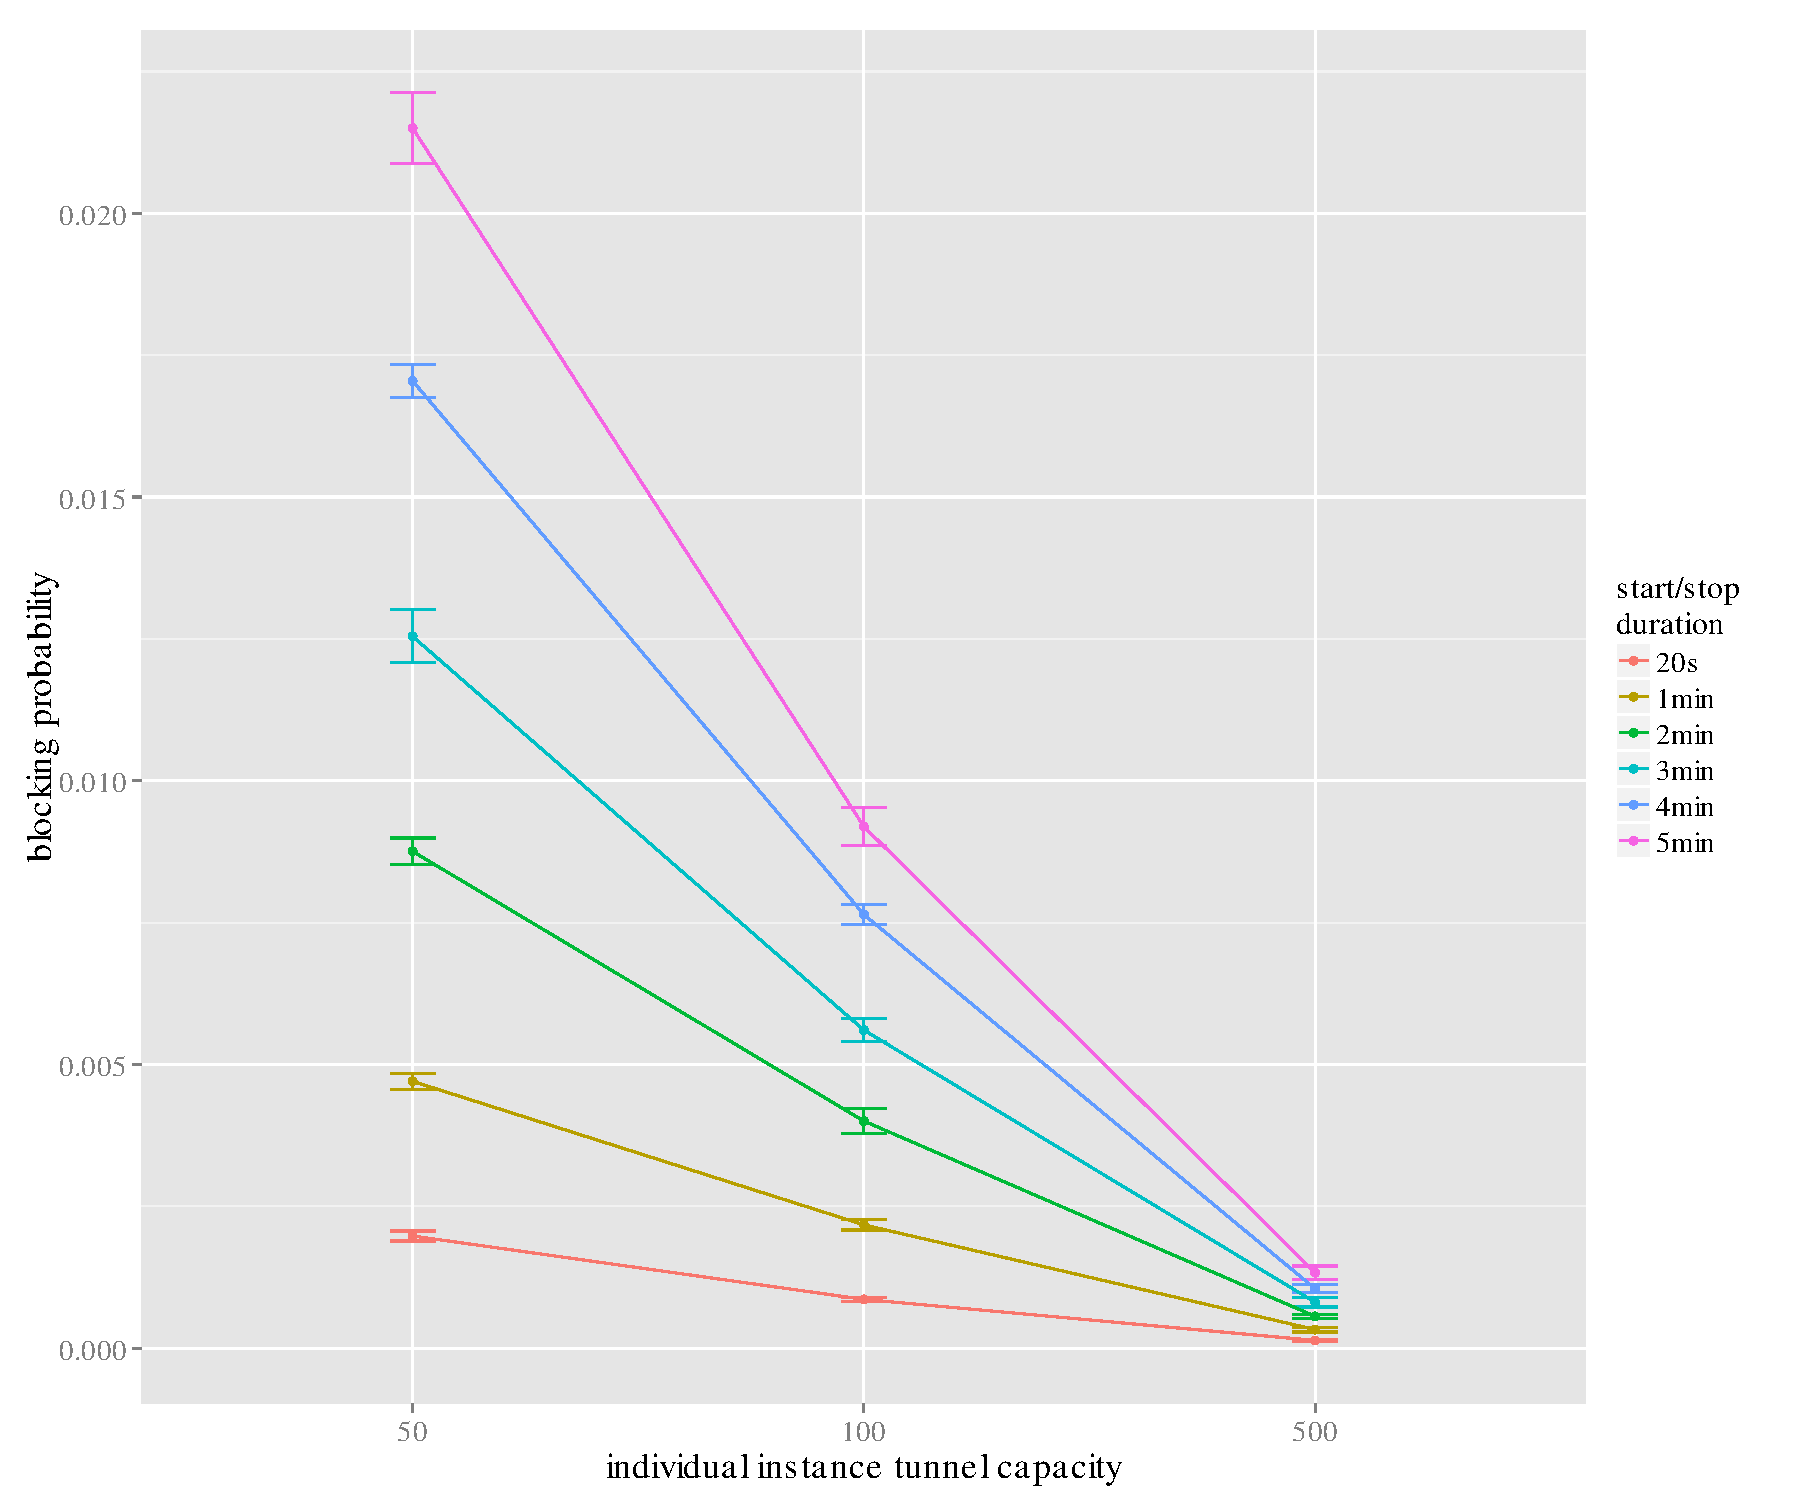
\includegraphics{images/compare-maxinstances-block.pdf}
  \caption{Influence of start up and shut down time on blocking probability with regard to different numbers of servers.}
 \label{c4:fig:compare_maxinstances_block}
\end{figure}

In order to study this behavior in more detail, we focus on a specific scenario in Figure~\ref{c4:fig:compare_maxinstances_block}, where $5000$ total tunnels should be supported by the system. In order to achieve this goal, we consider three types of instances, with the server capacity varying between $50$ and $500$.  In each case we change the start up and shut down time between $1$ and $5$ minutes. It can be easily observed, that lower server capacities combined with higher start up and shut down times increase the blocking probability. This is due to the server start up threshold mechanism, used in the model, not taking the additional capacity gained by activating an additional server into account. If a low capacity server with a long boot time is activated, there is a high probability that the system will quickly expend its capacity again.

Thus, it can be concluded, that if smaller instances are to be used, for example because they are cheaper than large instances, start up and shut down times should be kept minimal, for example by using virtual instances or \glspl{SSD}.




%%%%%%%%%%%%%%%%%%%%%%%%%%%%%%%%%%%%%%%%%%%%%%%%
% additional figures for simulation

\begin{figure}[htb]
  \centering
  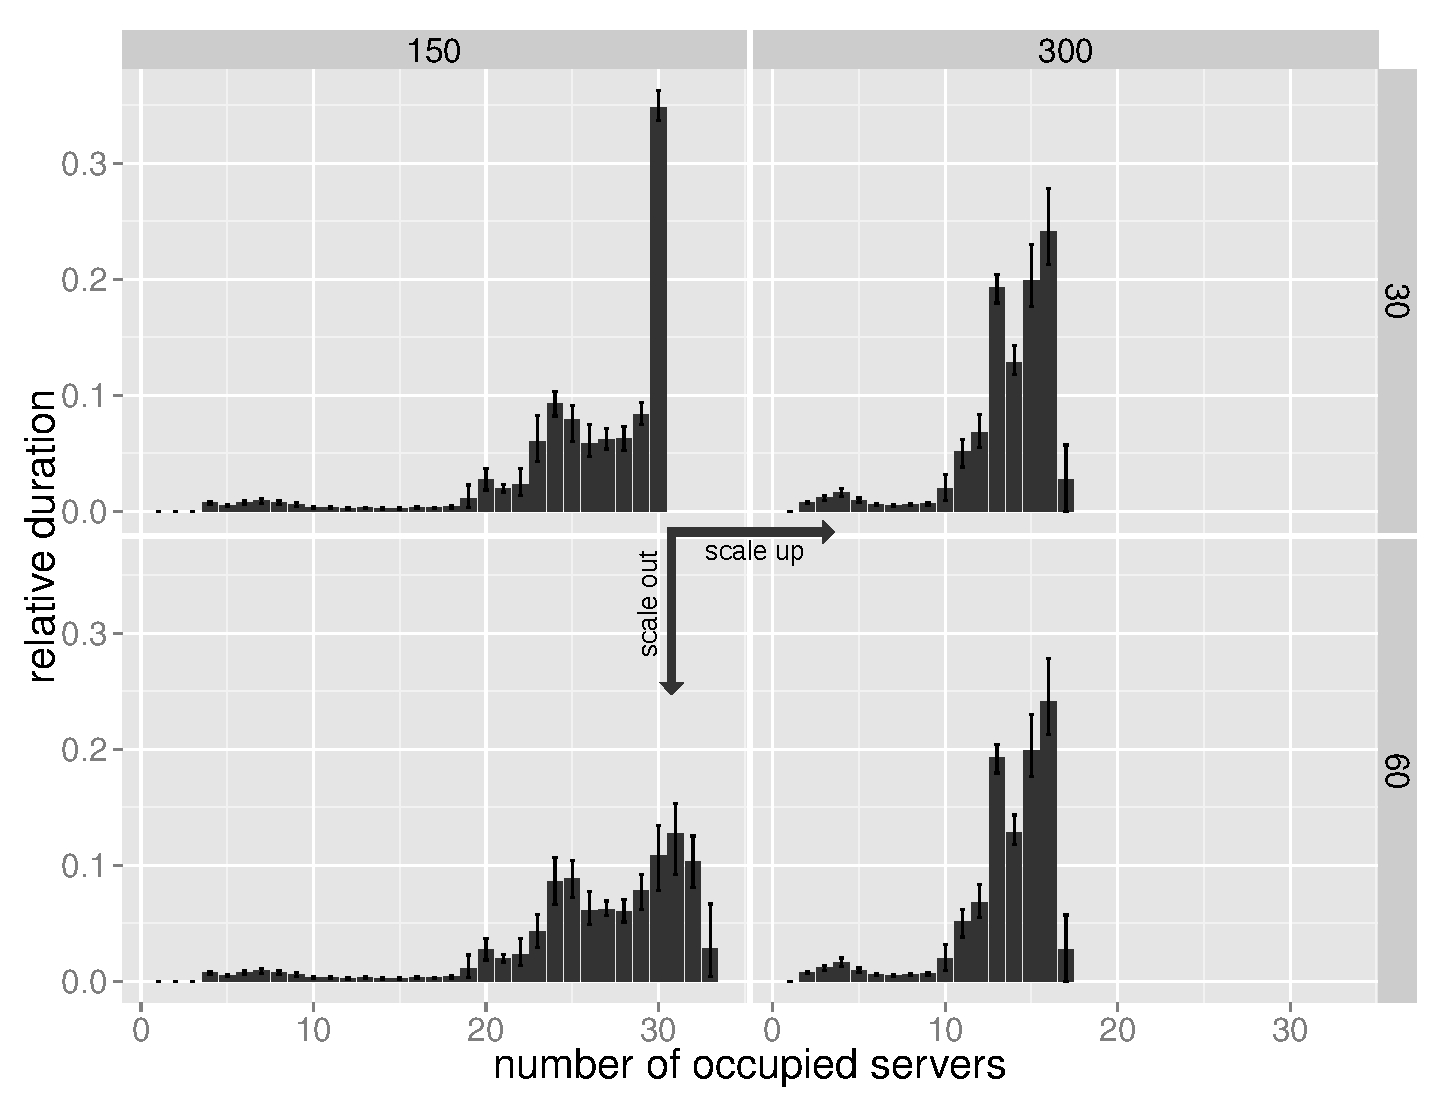
\includegraphics[width=1.0\textwidth]{images/resourceusedistribution-detail-barplot-annotated.pdf}
  \caption{Resource usage from select maximum instances and tunnels combination, displaying the capability to scale.}
 \label{c4:fig:res-usage-barplot}
\end{figure}


\begin{figure}[htb]
  \centering
  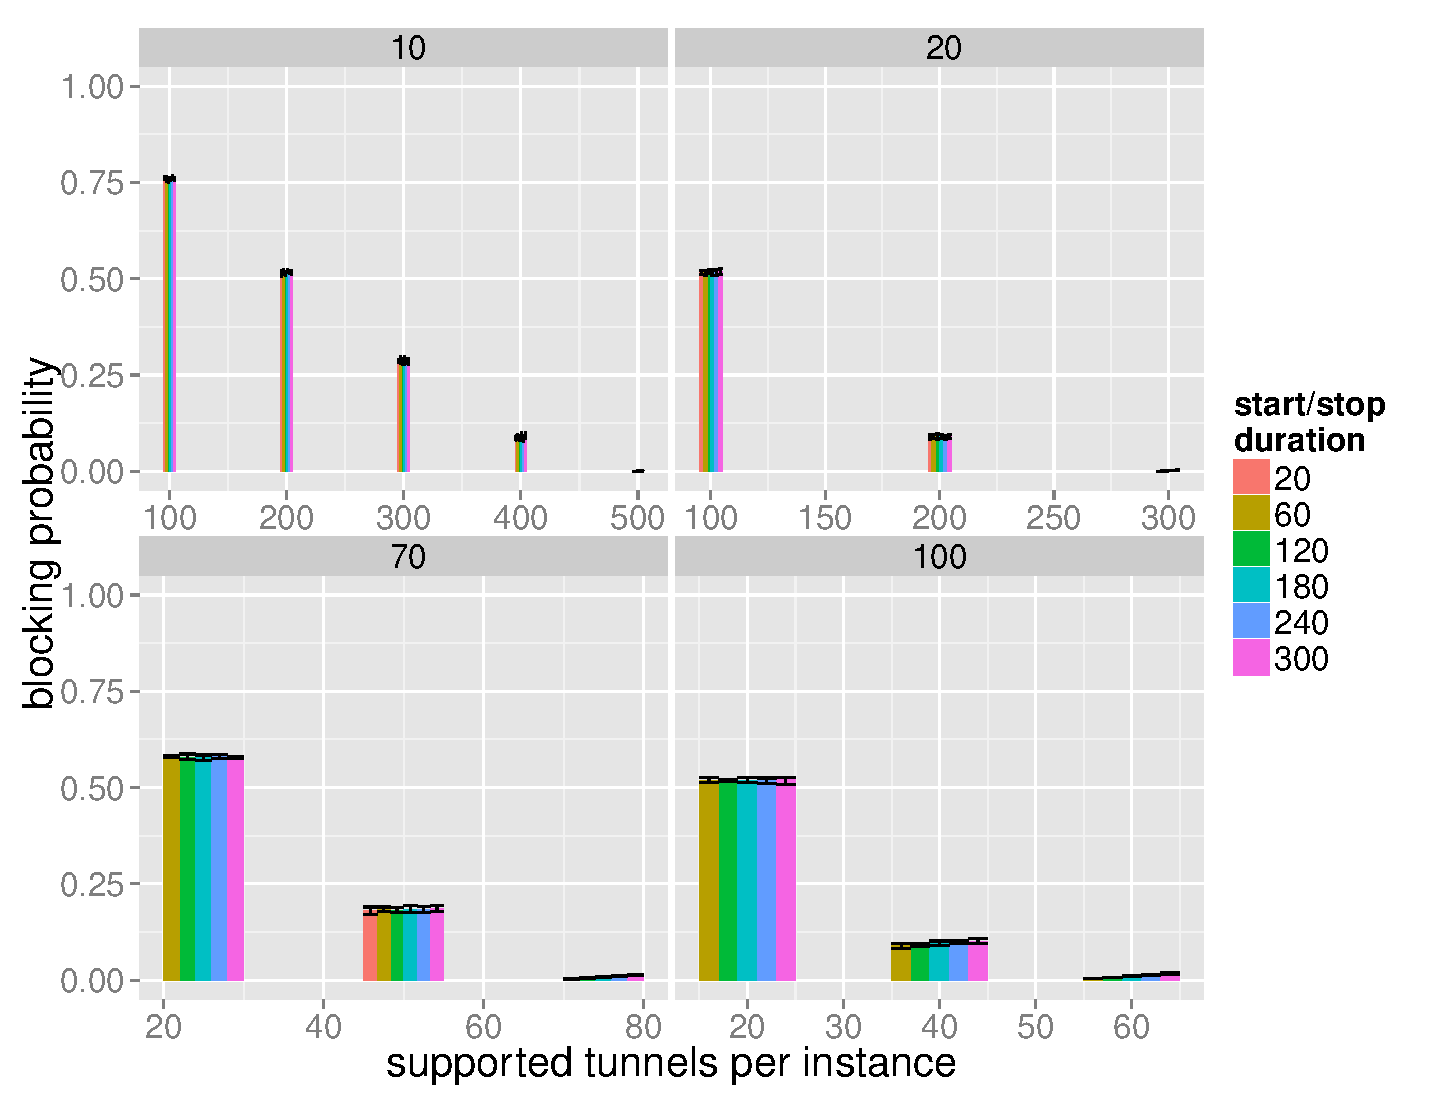
\includegraphics[width=1.0\textwidth]{images/startstopduration-blockingprobability-barchart.pdf}
  \caption{Influence of the boot and shutdown time on the blocking probability.}
 \label{c4:fig:blockprob-startstop-barchart}
\end{figure}

\begin{figure}[htb]
  \centering
  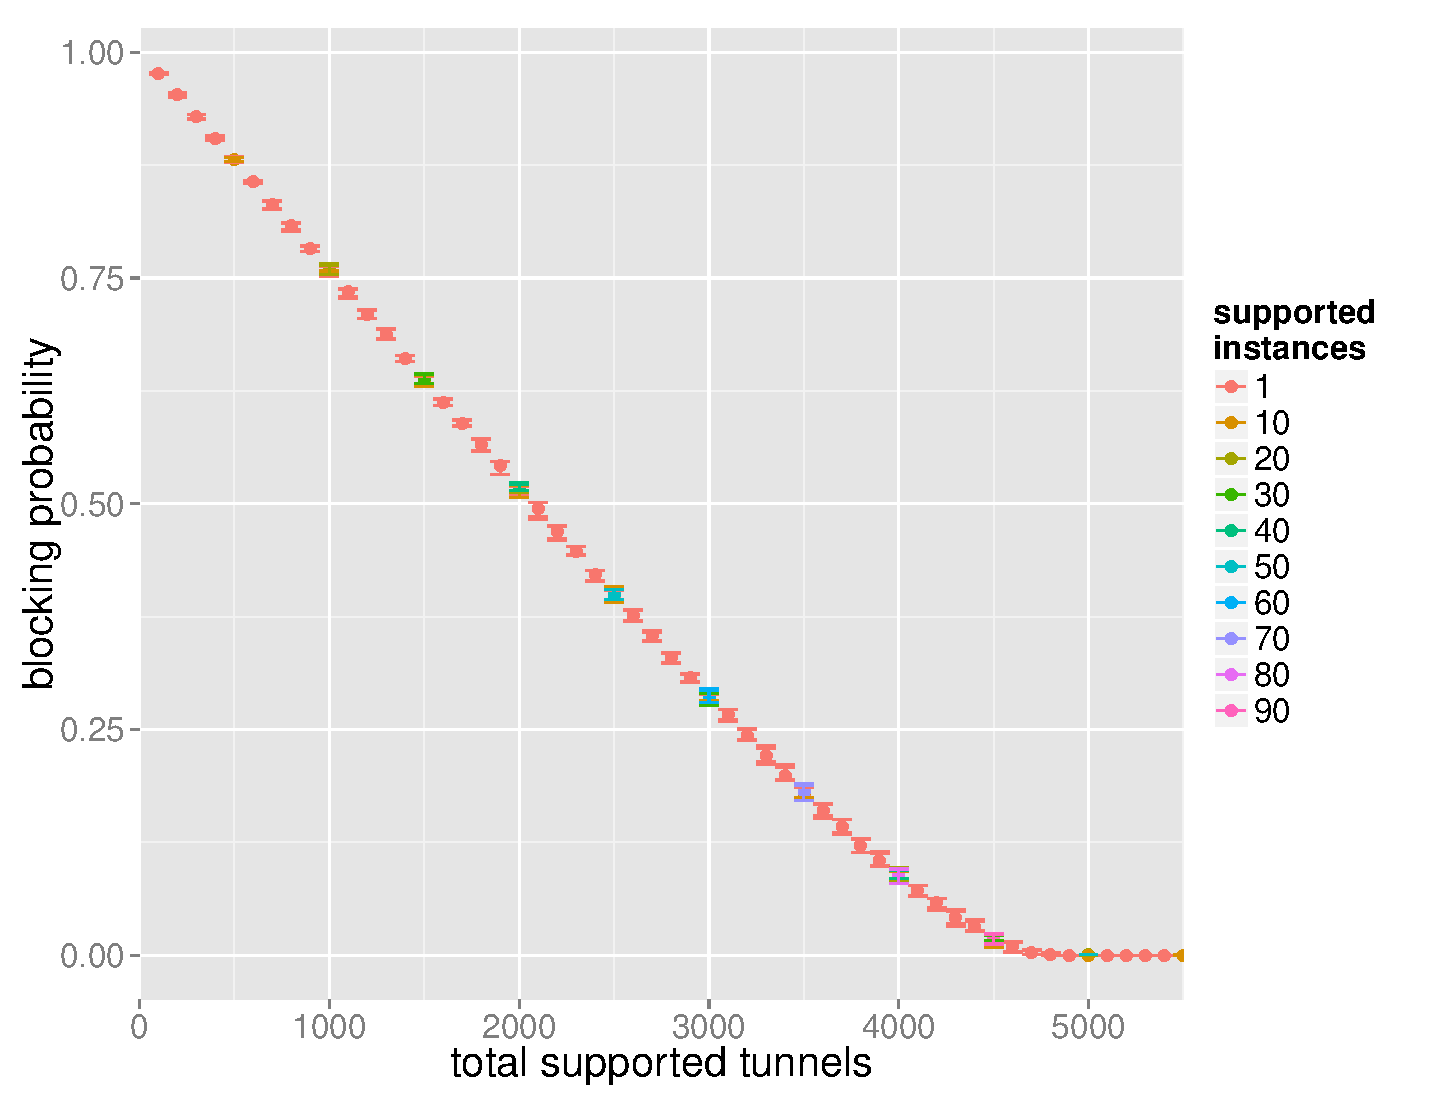
\includegraphics[width=1.0\textwidth]{images/feasiblemultiserver-blockprob.pdf}
  \caption{Comparison of the blocking probability of various server configurations.}
 \label{c4:fig:blockprob-multiserver}
\end{figure}

\begin{figure}[htb]
  \centering
  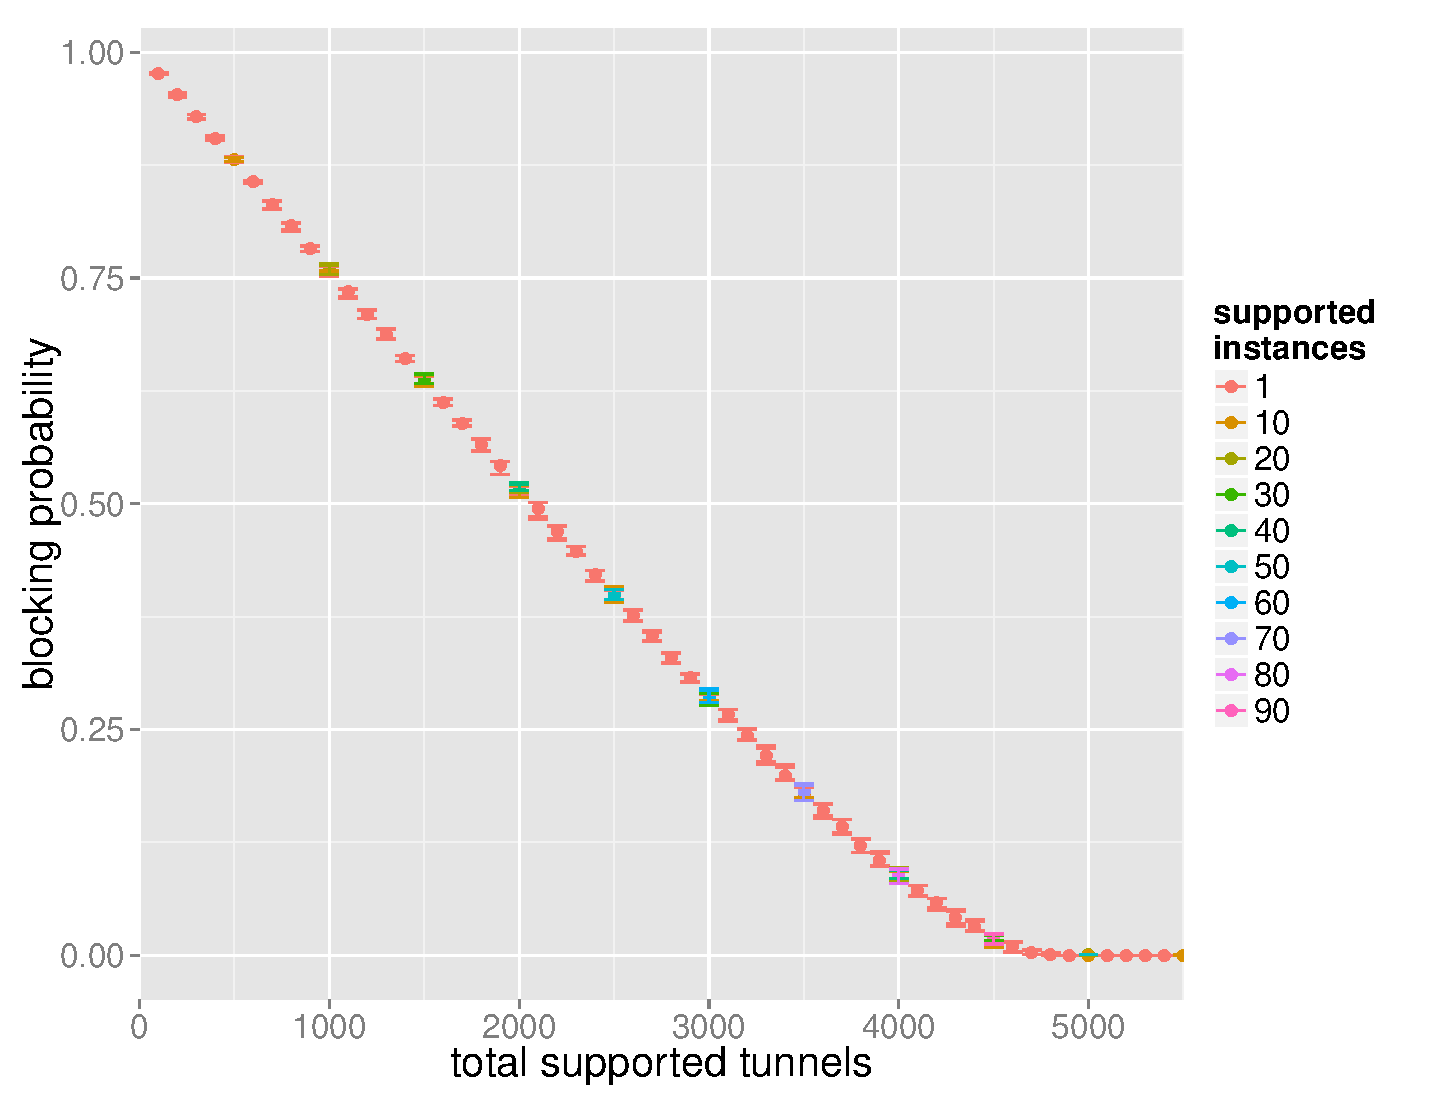
\includegraphics[width=1.0\textwidth]{images/feasiblemultiserver-blockprob.pdf}
  \caption{Comparison of the resource usage of various server configurations.}
 \label{c4:fig:res-usage-multiserver}
\end{figure}

\begin{figure}[htb]
  \centering
  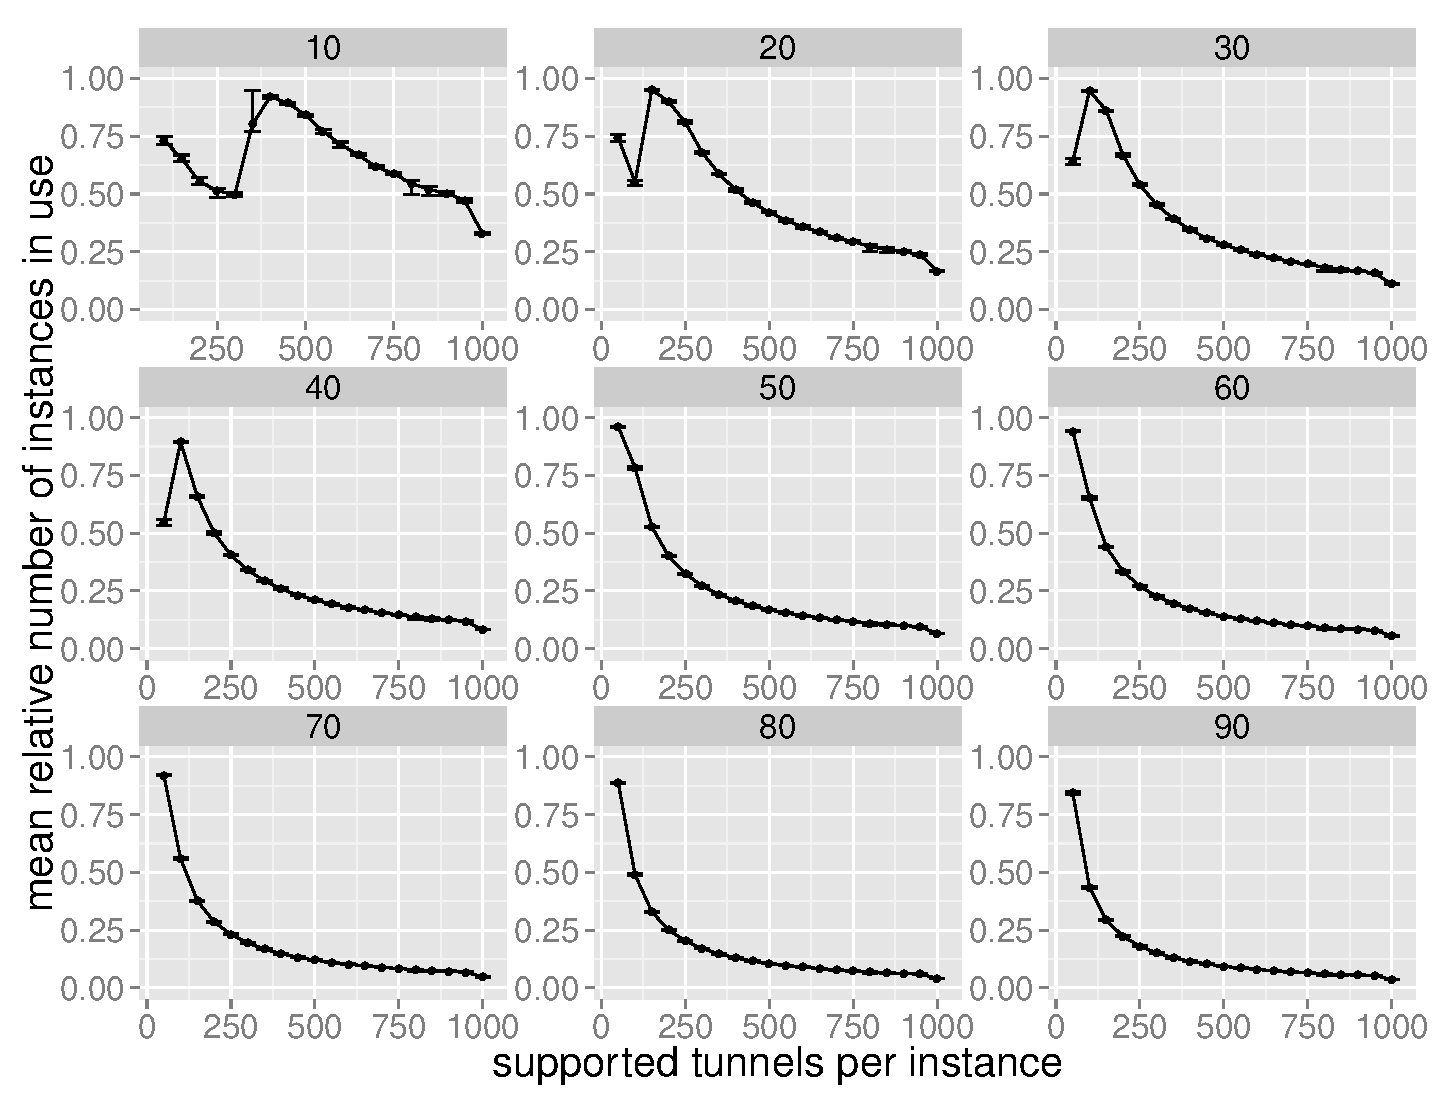
\includegraphics[width=1.0\textwidth]{images/instanceuse-mean.pdf}
  \caption{Mean instance usage of various server configurations.}
 \label{c4:fig:res-instance-usage-mean}
\end{figure}



%%%%%%%%%%%%%%%%%%%%%%%%%%%%%%%%%%%%%%%%%%%%%%%%%%%%%%%%%%%%%%%%%%%%%%%%%%%%%%%
\subsection{Modeling Discussion}

